\documentclass[ignorenonframetext, professionalfonts, hyperref={pdftex, unicode}]{beamer}

\usetheme{Copenhagen}
\usecolortheme{wolverine}

%Packages to be included
%\usepackage{graphicx}

\usepackage[russian]{babel}
\usepackage[utf8]{inputenc}
\usepackage[T1]{fontenc}

%%\usepackage[orientation=landscape, size=custom, width=16, height=9.75, scale=0.5]{beamerposter}

\usepackage{textcomp}

\usepackage{beamerthemesplit}

\usepackage{ulem}

\usepackage{verbatim}

\usepackage{ucs}


\usepackage{listings}
\lstloadlanguages{bash}

\lstset{escapechar=`,
	extendedchars=false,
	language=sh,
	frame=single,
	tabsize=2, 
	columns=fullflexible, 
%	basicstyle=\scriptsize,
	keywordstyle=\color{blue}, 
	commentstyle=\itshape\color{brown},
%	identifierstyle=\ttfamily, 
	stringstyle=\mdseries\color{green}, 
	showstringspaces=false, 
	numbers=left, 
	numberstyle=\tiny, 
	breaklines=true, 
	inputencoding=utf8,
	keepspaces=true,
	morekeywords={u\_short, u\_char, u\_long, in\_addr}
	}

\definecolor{darkgreen}{cmyk}{0.7, 0, 1, 0.5}

\lstdefinelanguage{diff}
{
    morekeywords={+, -},
    sensitive=false,
    morecomment=[l]{//},
    morecomment=[s]{/*}{*/},
    morecomment=[l][\color{darkgreen}]{+},
    morecomment=[l][\color{red}]{-},
    morestring=[b]",
}

\author[Epam]{{\bf Epam}\\Low Level Programming Department}

%\institution[EPAM]{EPAM}
%\logo{\includegraphics[width=1cm]{logo.png}}

\graphicspath{{../lvee2013-winter/clipart/}}
\title{Linux-образование \\ симбиоз ВУЗов, коммерческих компаний и LUG}
\author{Денис Пынькин, Юрий Адамов}

\begin{document}

\begin{frame}
	\titlepage
\end{frame}

\begin{frame}{Table of contents}
	\tableofcontents
\end{frame}


%%%%%%%%%%%%%%%%%%%%%%%%%%%%%%%%%%%%%%%%%   
%%%%%%%%%% Content starts here %%%%%%%%%%
%%%%%%%%%%%%%%%%%%%%%%%%%%%%%%%%%%%%%%%%%
\section[Проблема]{Проблема Linux-образования}
\mode<all>{\begin{frame}
	\frametitle{Задача бизнеса}

	\begin{block}{Заработать денег владельцам}

	В сфере встраиваемых и серверных решений под управлением ОС Linux:

	\begin{itemize}
	  \item Сегмент Linux стремительно растёт
	  \item Проекты есть, людей нет
	  \item Специалистов никто не готовит 
	  \item Специалисты уезжают
	  \item Люди не знают инструментальную среду Linux
	\end{itemize} 

      \end{block}
\end{frame}



\begin{frame}
	\frametitle{Почему нас так мало?}

	\begin{block}{Проблемы с изучением Linux в ВУЗах}
		\begin{itemize}
			\item Де-факто закрытый стек технологий на основе ОС Windows
			\item Отсутствует изучение профессиональных инструментов
			\item Нет практики совместной разработки
			\item Преподавателями игнорируются подходы, принятые в мире связанном со Свободным ПО
			\item Само наличие Linux в образовательном процессе является 
				заслугой исключительно отдельных лиц, работающих в ВУЗе
		\end{itemize}
	\end{block}
\end{frame}
  

\begin{frame}{Почему нас так мало?}
  \begin{block}{Сообщество. Открытое ли?}
    \begin{itemize}
      \item Кастовость
      \item Снобизм и псевдо 'элитарность'
      \item Сложность первоначального вхождения
    \end{itemize} 
  \end{block} \pause

  \alert{Т.е. те же болячки, что и у белорусского IT в целом}
\end{frame}


\begin{frame}
	\frametitle{Где взять Linux-специалистов?}

	\begin{block}{Источники}
		\begin{itemize}
			\item Система образования в РБ? \\
				LOL
				\pause
			\item Существующие специалисты? \\
				Циркуляция одних и тех же лиц.
				\pause
			\item Естественный приток энтузиастов? \\
				Слишком медленно.
		\end{itemize}
	\end{block}
        \pause
	\begin{block}{Решение}
		\begin{itemize}
			\item Самостоятельная планомерная подготовка специалистов
			\item Создание благоприятной экосистемы для самозарождения
		\end{itemize}
	\end{block}
\end{frame}


\begin{frame}[fragile]{Заинтересованные стороны}

	  \begin{itemize}
		\item MLUG
		\item EPAM Systems
		\item SaM-Solutions
		\item Promwad
		\item БГУИР
		\item БГУ
                \item ???
	  \end{itemize}


\end{frame}

}
\section{Сотрудничество}
\mode<all>{\begin{frame}{Collaboration Initiative}

  \begin{center}
    Мысли глобально, действуй локально

    
\includegraphics[height=0.6\textheight]{think-globally-act-locally}

    \begin{itemize}
      \item Инициатива сотрудников снизу
      \item Работаем через нейтральную открытую площадку
    \end{itemize}

  \end{center}

\end{frame}

\begin{frame}{Конкуренция между компаниями}
      
  \center\Large\alert{Конкуренции - нет}\footnote{См кол-во проектов и падение плотности специалистов}

  \center
\includegraphics[height=0.7\textheight]{penguin}

\end{frame}


\begin{frame}[fragile]{Ранняя публикация результатов}

  \begin{center}
    \alert{Release early, release offen} 

\begin{lstlisting}
  # find linux_courses/ -name "*.tex"|wc -l
  48
\end{lstlisting}

    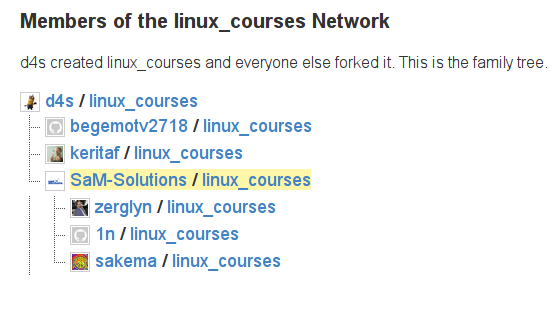
\includegraphics[width=0.65\textwidth]{members}

    \alert{Go github!}
  \end{center}
  
\end{frame}

\begin{frame}{Call for partnership}
  
  \begin{center}
    Открытый проект 'Linux образование' предлагает воспользоваться имеющимися материалами.
    
    
\includegraphics[width=0.6\textwidth]{copying}
  \end{center}

  А также с благодарностью примет:
  \begin{itemize}
    \item на хранение, распространение и доработку курсы
      \begin{itemize}
	\item незаконченные и готовые
	\item одноразовые и умершие
	\item осиротевшие
      \end{itemize}
    \item патчи
    \item баг-репорты
    \item pull-request'ы
  \end{itemize}

\end{frame}
}
\section[Epam]{Курсы по Linux от Epam}
\mode<all>{\begin{frame}{}
	\Huge
	\center{Developers!\\Developers!\\Developers!\\}
\end{frame}


\begin{frame}
	\frametitle{Developers! Developers! Developers!}

	\begin{block}{Цели}
		\begin{itemize}
			\item Увеличение популярности GNU/Linux среди программистов
			\item Воспитание потенциальных сотрудников
		\end{itemize}
	\end{block}

	\pause

	\begin{block}{Целевая аудитория}
		\begin{itemize}
			\item Студенты технических специальностей
			\item Любые программисты, желающие освоить работу в ОС Linux
		\end{itemize}
	\end{block}

	\begin{block}{Требования к кандидатам}
		\begin{itemize}
			\item Уже уметь программировать, под любую другую платформу.
		\end{itemize}
	\end{block}
\end{frame}

\begin{frame}
	\frametitle{Программа}

	\begin{block}{Командная строка -- важнейший инструмент понимания процесса разработки}
		\begin{itemize}
			\item Представление об архитектуре GNU/Linux дистрибутива
			\item Введение в shell-программирование
			\item Классические средства разработки, отладки и оптимизации
		\end{itemize}
	\end{block}
\end{frame}

\begin{frame}
	\frametitle{Первый набор}

	\center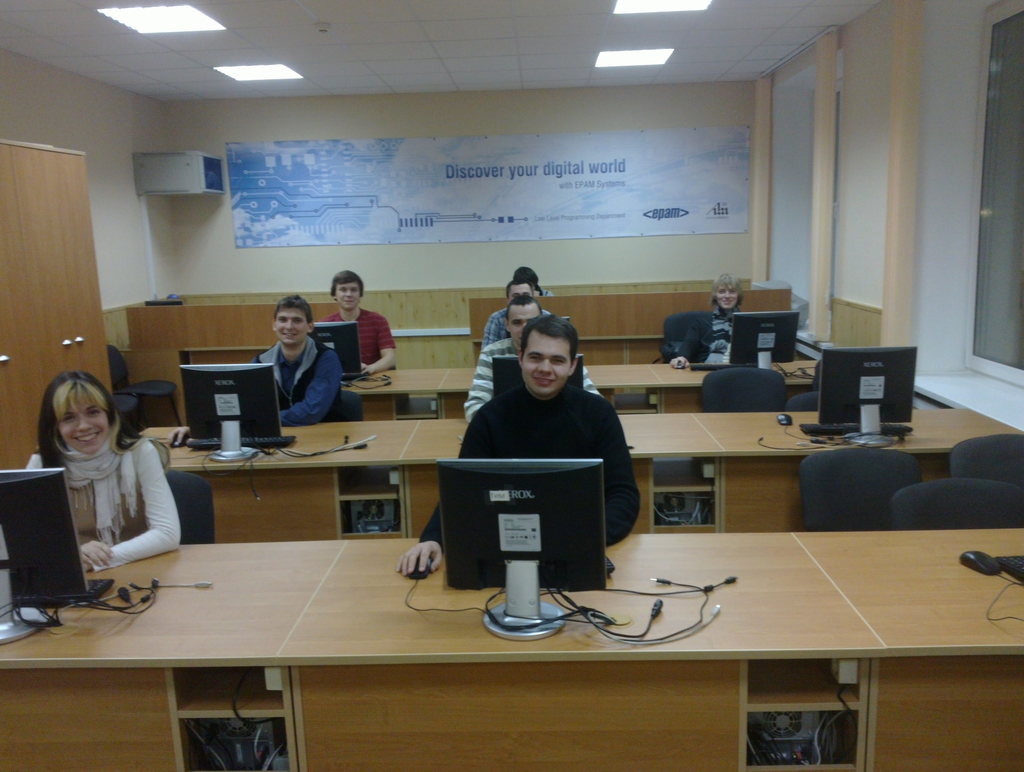
\includegraphics[height=0.5\textheight]{epam-evm_lab512}

	\begin{block}{Немного статистики}
		\begin{itemize}
			\item Подано заявок: {\bf 39} человек
			\item После первоначального отбора: {\bf 16} человек
				\begin{itemize}
					\item из них {\bf 4} -- сотрудники Epam
				\end{itemize}
		\end{itemize}
	\end{block}
\end{frame}

\begin{frame}
	\frametitle{Формат проведения занятий}

	\begin{block}{Принципы}
		\begin{itemize}
			\item Лекторы? Учителя? {\bf NO WAY!!!} 
				Разработчики для разработчиков! 
			\item Небольшая группа изучающих
			\item Балланс между теорией и практикой
		\end{itemize}
	\end{block}

	\pause

	\begin{block}{ $\beta$ -- версия: текущий статус}

		Все еще в \sout{разработке} процессе.

		\begin{itemize}
			\item Все планы нарушены ;-)
			\item 2 увлеченных человека
			\item Практически закончены 2 первых модуля
			\item Материалы выкладываются в общий доступ ``по-готовности''
				\begin{itemize}
					\item Патчи от студентов уже есть
				\end{itemize}
		\end{itemize}
	\end{block}

\end{frame}


\begin{frame}
	\frametitle{Планы}

	\begin{block}{Сила в сообществе}

		\begin{itemize}
			\item Развитие взаимодействия с open-source сообществом
			\item 
		\end{itemize}
	\end{block}


\end{frame}

\begin{frame}
	\frametitle{}

\end{frame}

\begin{frame}
	\frametitle{}

\end{frame}

\begin{frame}
	\frametitle{}

\end{frame}

}
\section{Развитие проекта}
\begin{frame}[fragile]{Эволюция}

  \begin{columns}

	  \column{0.35\textwidth}

	  \begin{center}
		{\Large февраль 2013}
	  \end{center}

	  \begin{itemize}
		\item 6 авторов
		\item 177 коммитов
		\item 1.5 курса
	  \end{itemize}

	  \begin{itemize}
		\item MLUG
		\item Epam (БГУИР)
		\item SaM-Solutions
		\item[]
	  \end{itemize}

    \column{0.35\textwidth}

	  \begin{center}
		{\Large январь 2014}
	  \end{center}

	  \begin{itemize}
		\item 14 авторов
		\item 312 коммитов
		\item 3.5 курса
	  \end{itemize}

	  \begin{itemize}
		\item MLUG
		\item Epam (БГУИР)
		\item SaM-Solutions
		\item Promwad (БГУ)
	  \end{itemize}

  \end{columns}

\end{frame}
\begin{frame}{Call for partnership}
  
  \begin{center}
    Открытый проект 'Linux образование' предлагает воспользоваться имеющимися материалами.
    
    
\includegraphics[width=0.6\textwidth]{copying}
  \end{center}

  А также с благодарностью примет:
  \begin{itemize}
    \item на хранение, распространение и доработку курсы
      \begin{itemize}
	\item незаконченные и готовые
	\item одноразовые и умершие
	\item осиротевшие
      \end{itemize}
    \item патчи
    \item баг-репорты
    \item pull-request'ы
  \end{itemize}

\end{frame}
\begin{frame}[fragile]{}

  \Large \alert{Вопросы?}  \footnote{Авторы благодарят ex-сотрудника компании SaM-Solutions \\
  Влада (mend0za) Шахова за использованные при подготовке материалы}

  \bigskip

  \href{http://mlug.linux.by}{http://mlug.linux.by}

  \href{https://github.com/epam-llpd/linux\_courses}{https://github.com/epam-llpd/linux\_courses}

  \hrulefill

  \href{mailto:denis\_pynkin@epam.com}{denis\_pynkin@epam.com}

  \href{mailto:yury\_adamov@epam.com}{yury\_adamov@epam.com}


\end{frame}

\end{document}
